\documentclass[sigconf, 7pt]{acmart}

\usepackage{graphicx}
\usepackage{stfloats}

\settopmatter{printacmref=false} % Removes citation information below abstract
\renewcommand\footnotetextcopyrightpermission[1]{} % removes footnote with conference information in first column
\pagestyle{plain} % removes running headers

\title{\textbf{Optimal Optimization of the Non-Quadratic Sphere}}
\author{Ravinder Rai}
\date{\today}


\begin{document} 


\begin{abstract}
In this report, we compare two different types of optimization algorithms, a quasi-newton algorithm and an evolution strategy algorithm. Both algorithms seek to solve the problem of finding a minimum value of a specific variant of the sphere, namely the non-quadratic sphere. We compare these algorithms by comparing the number of function evaluations used to find the minimum value of the sphere, given certain parameters. The results are collected by varying a certain parameters one at a time, and are displayed on one plot per parameter. One of two main results that is expected and explored here is that, as dimension increases, the cost (number of function evaluations) should increase as well. The second main result then shows how different powers of this variant of the sphere can affect the cost, and what algorithm is best used to minimize this cost.
\end{abstract}
\maketitle

\section{Introduction}
\label{sec:intro}

In this paper, we compare the cost of two optimization algorithms to find the minimum value of a certain test problem, that being the non-quadratic sphere. The first of the two algorithms is a quasi-newton algorithm, and is implemented by using a Matlab function, fminunc. The second of the two algorithms is an evolution strategy algorithm, called the $(1+1)$-ES algorithm. When experimenting with both of these functions, we vary certain parameters and observe how the changes affect the optimization results, specifically the cost as it relates to the number of function evaluations. This report shows how increasing dimension and the exponent of the sphere can increase the cost of optimizing the problem. We expect that increasing both dimension and the exponent of the sphere simply increases the number of function evaluations. 


\section{Preliminaries}
\label{sec:pre}
Here we highlight some important tools used in this paper, the most important being the fminunc function in Matlab. This function tries to minimize a given function/test problem (with no constraints), which in this case was a variant of the sphere function. The fminunc function follows one of two algorithms, one being the trust-region algorithm, and the other being the quasi-newton algorithm. The quasi-newton algorithm is the algorithm of interest here, so by simply not supplying fminunc with gradients, it automatically uses this desired algorithm. The quasi-newton algorithm works by starting with some initial $x$ value, and making steps in some direction to find a local minimum. It does this by approximating the Hessian matrix, and uses it to make optimal steps in the direction that would give the minimum function value. The Hessian matrix approximation is updated as the algorithm iterates, but there are three different ways to update the Hessian, and all three of these Hessian updates give different results. When comparing this algorithm with the $(1+1)$-ES algorithm, all different Hessian update variants will be shown in the final plots. Also, note that the $(1+1)$-ES algorithm differs from fminunc, in that it does not use a Hessian, and simply checks (and compares) function values at every iteration, and follows a certain update (explained below) in a step by step process until some target value is reached. As mentioned previously, the non-quadratic sphere is the test problem here and is of the form: $f(x)=(x^tx)^{\beta/2}$, where $x$ is an $n$ dimensional column vector. $x^t$ represents the transpose so that $x^tx$ becomes the dot product, giving a scalar value. The sphere becomes non-quadratic when we introduce and vary the value of $\beta$, which is one of two main parameters to vary (the other being the dimension, $n$).




\section{Algorithm}
\label{algorithm}
There are two algorithms used to get the results below, both designed to actually complete the minimization of the non-quadratic sphere. The first algorithm is the quasi-newton algorithm, given by the fminunc function in Matlab. We first start with an initial starting point, $x_0$ (an $n$ dimensional column vector with random elements belonging to a normal distribution). Then we set our options for Matlab's fminunc function, which include the Hessian update option, the maximum number of function evaluations allowed, the optimality tolerance, and a few others. We are only interested in achieving target values here, so we set these options to be either arbitrarly small or large, depending on the option, to ensure that fminunc stops and only stops when the function value is below the given target. Next, we define a function that stores necessary variables, like function values for instance, for plotting purposes. Finally we define the objective function, which is the non-quadratic sphere as defined above. Overall, this function will take arguments: $n$ for the dimension, $\beta$ for the power, a target function value, and the Hessian update (a string), and returns the variables that we recorded. Note, some of the code to implement this was borrowed from \cite{MathWorks}.

The second algorithm is the $(1+1)$-ES algorithm, and it works as follows: first pick initial points, $x_0$ (chosen as in the previous algorithm) and $\gamma$, and then define $y = x + z*\gamma$, where $z$ is a vector with random elements from a normal distribution, and gamma is some update variable. Then, if the function value at $y$ is less than the function value at $x$, set $y$ to be the new $x$ and multiply gamma by $e^{(0.8/n)}$, and if not, then multiply gamma by $e^{(-0.2/n)}$. This $\gamma$ update is called the $1/5$ rule, and it works well because when we achieve a better $x$ value (such that $f(x)$ is smaller than the previous $f(x)$), $\gamma$ will increase in step size, and in the other case, $\gamma$ will decrease so that the step size does also.  This process is repeated until a specified target value is reached. Throughout this process we count and record the number of function evaluations as well as the function values for later plotting. Finally, using both of these functions, we can iterate through chosen values of $\beta$ and $n$ to display plots of the number of function evaluations against these varying parameters. $\gamma$ will be set to a value of $1$ for all experiments to keep observing the other parameters simple. We know the minimum value of the non-quadratic sphere is zero, so the target here is set to $1e-6$ for all runs.



\section{Results and Discussion}
\label{result}


\begin{figure}[h]
\centering
  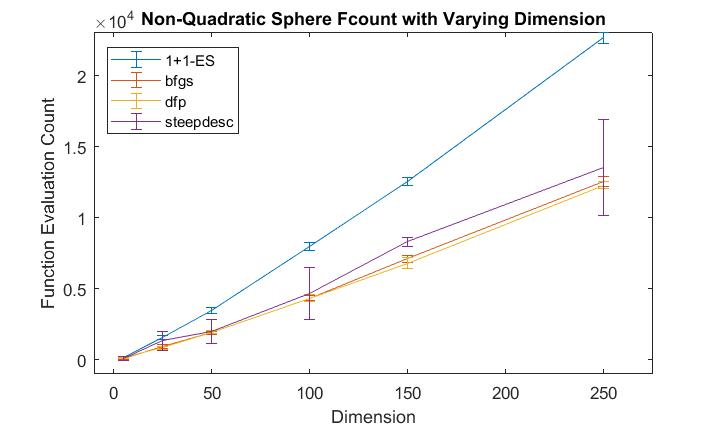
\includegraphics[height = 5.5cm, width=9cm]{A2DimFcount.jpg}
  \caption{This plot displays the number of function evaluations of various optimization algorithms as the dimension, $n$, increases. $\beta = 10$ for each plot. The plotted dimension values are $n=5, 25, 50, 100, 150, 250$}
  \label{fig:sdimen}
\end{figure}

The first result is shown in Figure \ref{fig:sdimen}, and shows how increasing the dimension affects the non-quadratic sphere. In this case, we kept $\beta = 10$ constant, to accurately view the affect of the dimension on the problem. The data presented here is the median of several runs, to get reproducible results, and the error bars indicate the spread, taken from the maximums and minimums from all the runs. You can see that increasing the dimension of the problem did have the expected result, being that higher dimensions would simply increase the number of function evaluations for both the fminunc function (with all of its' Hessian update variants) and the $(1+1)$-ES algorithm. More importantly, it is clear that the number of function evaluations for the $(1+1)$-ES algorithm is the highest, while the fminunc function is less, with all three Hessian update variants giving similar results. 

\begin{figure}[h]
\centering
  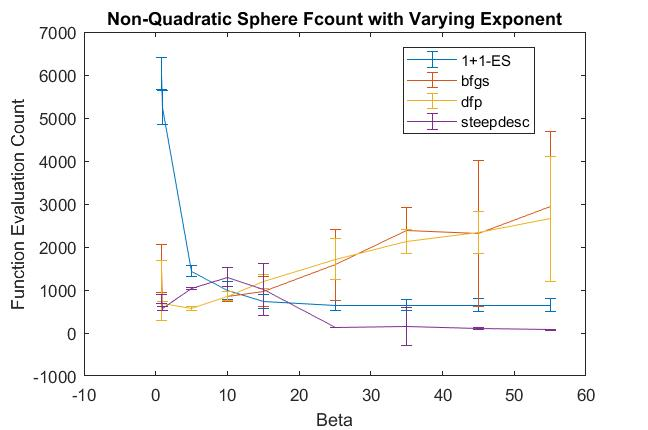
\includegraphics[height = 5.5cm, width=9cm]{A2BetaFcount.jpg}
  \caption{This plot displays the number of function evaluations of various optimization algorithms as the exponent, $\beta$, increases. The dimension for each plot is $n = 25$. The plotted $\beta$ values are $\beta = 0.75, 0.9, 5, 10, 15, 25, 35, 45, 55$}
  \label{fig:beta}
\end{figure}

Next, Figure \ref{fig:beta} shows a similar result, except now the varying parameter is $\beta$. The results in this plot are more interesting, because you can see that as the value of $\beta$ increases, the number of function evaluations for the $(1+1)$-ES algorithm decreases exponentially. This may be due to the $1/5$ rule that was applied to the $\gamma$ update, because it appears in the equation to calculate the $y$ values in the algorithm, which then gets raised to the power of $\beta/2$. So for large values of $\beta$, the exponential factor may be a dominate part of the $y$ value thus causing an exponential decay. This is especially evident with the smaller exponents ($\beta < 1$), where the number of function evaluations are much larger than for $\beta \geq 1$. As for the fminunc results, it appears to simply be a linear increase in the number of function evaluations, but only for the Hessian variants bfgs and dfp. The steepest descent Hessian variant seems like it has linear increase at the beginning of the plot, but then plateaus at around zero. This is because the fminunc function failed to solve the problem, and stopped too early, thus resulting in a very low number of function evaluations. In fact, the bfgs and dfp Hessian variants also give the same error for $\beta$ values outside of the interval in Figure \ref{fig:beta}. You can see this in the spread for the larger values of $\beta$, as the error bars are much larger because some of the runs failed too early, resulting in lower function evaluation counts, which then get recorded as the minimum in the error bars. Decreasing the dimension may help deal with numerical issues and allow plotting larger $\beta$ values, but the dimension is already relatively small here, so not much more can be done.

These results shows that the $(1+1)$-ES algorithm is probably the better choice when optimizing the non-quadratic sphere, but more so with larger parameter values (specifically $\beta$). However, the results from Figure \ref{fig:sdimen} suggest otherwise, in that with constant $\beta$ values, fminunc does better with higher dimensions. Finally, Figure \ref{fig:beta} further suggests that fminunc may be better for much values of $\beta$, as the cost is quite high when using the $(1+1)$-ES algorithm, but if you go too small then fminunc may run into numerical issues, and in this case there is no other choice but to use the $(1+1)$-ES algorithm.


\section{Conclusion}
\label{con}
From the results observed in Figure \ref{fig:sdimen} and \ref{fig:beta}, the $(1+1)$-ES algorithm seems to be the best option for larger parameter values since it does not fail like fminunc, and even has a lower cost with larger $\beta$ values. That being said, it also appears that for smaller dimensions the $(1+1)$-ES algorithm may be the worst choice out of the presented options, and fminunc with any Hessian variant would be better. Furthermore, since the number of function evaluations decreases at an exponential rate as $\beta$ increases for the $(1+1)$-ES algorithm, it appears that this would algorithm should always work well for large values of $\beta$, but the cost will level out. For future exploration, it may be of interest to try different values of $\gamma$, thus changing the initialization conditions to get better results for the $(1+1)$-ES algorithm. Other evolution strategies would also be interesting to plot alongside the algorithms here.

\begin{thebibliography}{9}
\bibitem{MathWorks} 
MathWorks Output Functions,
\\\texttt{https://www.mathworks.com/help/releases/R2015b/optim/ug/output-functions.html}
\end{thebibliography}


\end{document}